\documentclass[11pt, oneside]{article} 
\usepackage{geometry}
\geometry{letterpaper} 
\usepackage{graphicx}
	
\usepackage{amssymb}
\usepackage{amsmath}
\usepackage{parskip}
\usepackage{color}
\usepackage{hyperref}

\graphicspath{{/Users/telliott/Dropbox/Github-Math/quickgeo/figures/}{/Users/telliott/Dropbox/Github-Math/figures/}}
% \begin{center} \includegraphics [scale=0.4] {gauss3.png} \end{center}

\title{Thales' theorems}
\date{}

\begin{document}
\maketitle
\Large

%[my-super-duper-separator]

\subsection*{circles}

\begin{center} 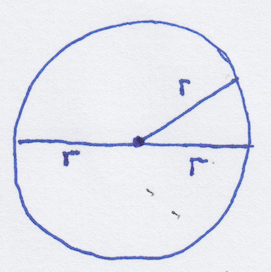
\includegraphics [scale=0.5] {B11.png} \end{center}

The easiest way to draw a circle is to just pick some point to be the center.  Then draw all the points that lie a given distance away from the center.  That distance is called the radius, $r$.

$\circ$  \ All the points on the circle are equidistant (the same distance) from the center.

That is not a theorem but an axiom, something that we choose to believe about the world.

A diameter is a straight line through the center, and since each half is a radius, the diameter $d = 2r$.

Thales (624-546 BC) was from a Greek town called Miletus on the coast of Asia Minor (modern Turkey).  He lived long before Euclid --- about 300 years before.  Unfortunately, neither his writing nor an extensive history that was written later survives. 

The following is one of three elementary but novel theorems for which he is thought to have developed proofs.

\subsection*{Triangle sum theorem}

We did this one previously so we could use it before this, but Thales' proof is beautiful.

$\bullet$  The angle sum of a triangle is equal to two right angles.

\begin{center} 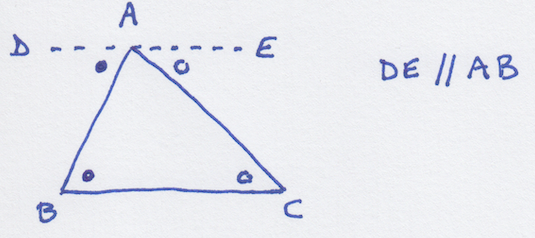
\includegraphics [scale=0.5] {D1.png} \end{center}

\emph{Proof}.

Draw a line segment through the top vertex of the triangle parallel to the base.  

Now, use alternate interior angles.  By the theorem, the two angles marked with filled circles are equal, as are the two angles marked with open circles.

The three angles under the top red line add up to two right angles, by the supplementary angle theorem.  So the total measure of three angles in a triangle is equal to two right angles.

Again, we put a little box to show that the proof is complete.

$\square$

The triangle sum theorem is very closely related to the parallel postulate.  There, we said that for a traversal of two parallel lines, which never meet, the sum of the internal angles is 180.  The converse would be that if the two lines did meet, somewhere far away, then we would have a triangle.  

Meeting at a third angle means that the sum of the internal angles must be less than 180, by the triangle sum theorem, since we must leave some (small) part of the 180 for the far distant angle.

\subsection*{Thales circle theorem}

Draw a circle and its diameter $AOC$ (actually, only a semi-circle is required, as we see here.

\begin{center} 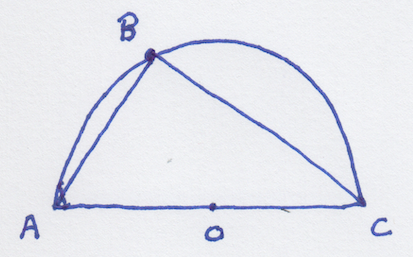
\includegraphics [scale=0.5] {D2.png} \end{center}

Pick any point on the periphery, $B$, and draw $AB$ and $BC$.  I claim that $\angle ABC$ is a right angle.

\emph{Proof}.

Draw $BO$.

\begin{center} 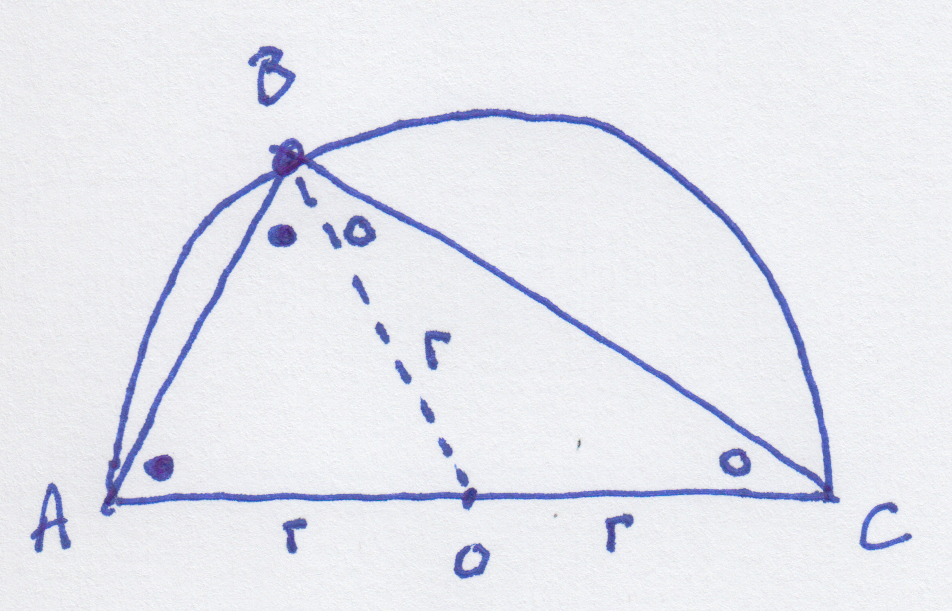
\includegraphics [scale=0.9] {D3.png} \end{center}

Since $AO$ is on the diameter, it is a radius of the circle.  $OB$ is also a radius, so they are equal.  Therefore $\triangle AOB$ is isosceles.  By the isosceles triangle theorem, the angles marked with filled dots are equal.

But then the two base angles of $\triangle BOC$ are also equal, by the same reasoning.

The sum of the two angles at vertex $B$ is one-half the sum of all the angles in the original triangle $ABC$.  Therefore $\angle ABC$ is a right angle.

$\square$

\subsection*{Converse of Thales circle theorem}

We showed above that given a diameter of the circle and any point on the circle (not on the diameter), the angle formed with the sides drawn from the diameter is a right angle.

We are now given that the angle at $P$ is a right angle, and $\triangle APB$ has $AB$ as a diagonal of the circle centered at $O$ with radius $AO$.  

We will prove that $P$ must be on the circle.

\begin{center} 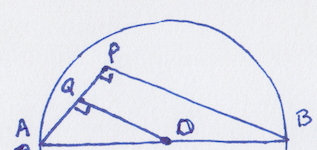
\includegraphics [scale=0.7] {D3c.png} \end{center}

\emph{Proof}.

Draw the perpendicular at $Q$ so that it goes through the center of the circle at $O$.  By similar triangles (three angles equal), $\triangle APB \sim \triangle AQO$ and since $AO$ is one-half the diameter, the ratio of sides is 2:1.

Using that ratio, $AQ = QP$.  (Note:  this step uses similarity and ratios of sides, which we won't prove for a few more chapters).

But this means that $\triangle AQO \cong \triangle POQ$, so $AO = OP$.  Thus, $\triangle AOP$ is isosceles.

But $AO$ is a radius of the circle, so $OP$ is also.  Therefore, $P$ must lie on the circle.

$\square$

We will prove the previous theorem again, in order to give a first proof by contradiction.  

In this method, we assume something that is the opposite of what we think may be true, and want to prove.  Then follow the logic until we reach a contradiction.  This logical dead end implies that the original assumption was incorrect, so the converse of the original statement is true.

We have the same situation but a slightly different diagram.  If $\angle APB$ is a right angle and $AB$ is a diameter, then $P$ is on the circle.
\begin{center} 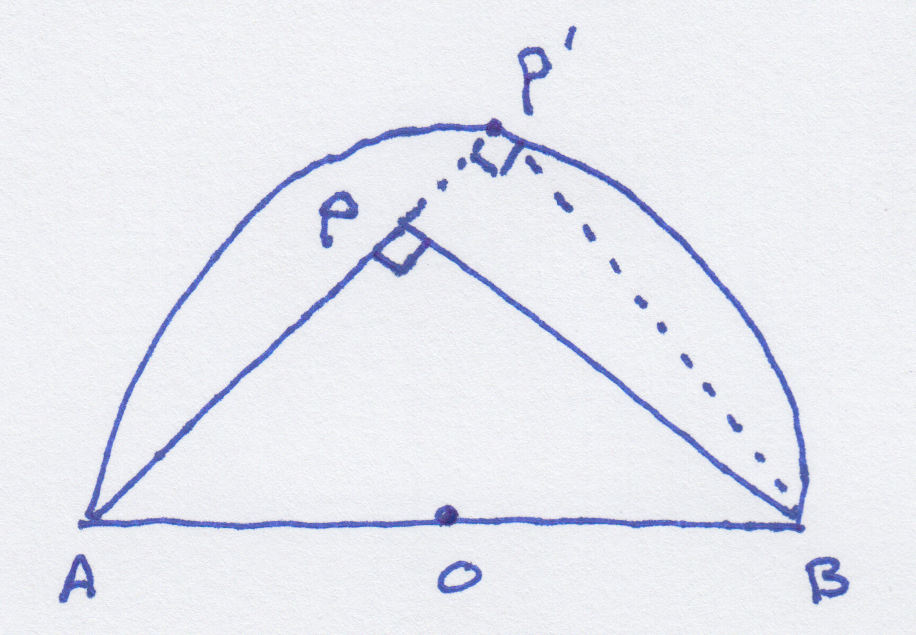
\includegraphics [scale=0.8] {D3b.png} \end{center}

\emph{Proof}.

By contradiction.  Assume that $\angle APB$ is a right angle, but $P$ lies inside the circle.

Draw the continuation of $AP$ to form $AP'$ with $P'$ on the circle.  Then, by the forward version of the theorem, $\angle AP'B$ is a right angle.  

We assumed that $\angle APB$ is also a right angle.  Therefore, by the parallel postulate, $PB$ is parallel to $P'B$.  

But these two line segments meet at $B$ so they are not parallel.  This is a contradiction.  

Therefore our assumption that $APB$ lies inside the circle was mistaken.

A similar argument shows that $P$ is not outside the circle, either.  If it does not lie either outside or inside the circle, it must lie on the circle.

$\square$

Since the converse is true, we know that \emph{any} right triangle can be embedded in a semicircle.

\subsection*{exterior angle theorem}

The form of the exterior angle theorem that we will use most often says that the angle $u'$ is equal to $s + t$.
\begin{center} 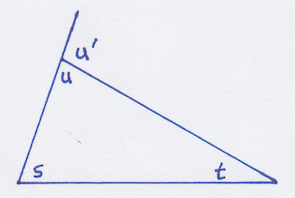
\includegraphics [scale=0.6] {D4a.png} \end{center}

\emph{Proof}.

$u'$ is supplementary to $u$, but the sum $s + t$ is supplementary also.  Therefore $u'$ is equal to $s + t$.

$\square$

A longer proof gives some more detail on the components of the exterior angle, although honestly, it is really just a repeat of the triangle sum theorem with the alternate interior angles theorem added in.

\emph{Proof}

Draw a triangle and extend one side.  Also draw a line segment at that vertex parallel to the opposite side.
\begin{center} 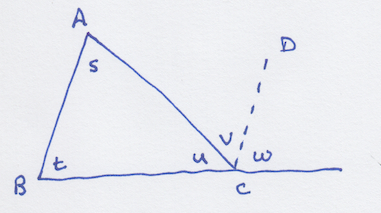
\includegraphics [scale=0.6] {D4b.png} \end{center}

The exterior angle at vertex $C$ is the sum of the two angles $v + w$.  These are equal to the opposing angles $s$ and $t$ because

\[ s + t + u = 180 = u + v + w \]
\[ s + t = v + w \]

Also $s = v$, by alternate interior angles, so $t = w$, by subtraction.

The exterior angle at any vertex is equal to the sum of the two internal angles on the side facing that vertex.

$\square$

Technically, the exterior angle theorem refers to Euclid's proof of a weaker result, which was that the exterior angle is greater than either one of the two internal angles on the side facing that vertex.  

His proof has been discussed \emph{a lot}, mainly because it is closely related to the parallel postulate.  We don't need to get off track by doing that here.  Proposition 32 of book 1 is equivalent to what we've done here.

\subsection*{beyond Thales}

Let us go back to Thales theorem about the right angle on a diameter of the circle.
\begin{center} 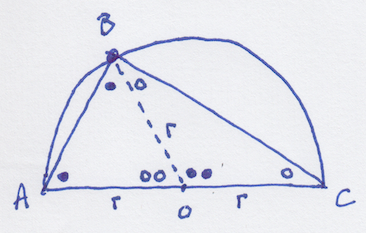
\includegraphics [scale=0.6] {D5.png} \end{center}
Fill in the measures of the central angles at $O$, using the exterior angle theorem from above.

We notice something interesting:  the angle at vertex $A$ is exactly one-half the central $\angle BOC$, and they cut off (subtend) the same arc on the circle.

This is a special case, because both $A$ and $O$ lie on the diameter.  But we begin to wonder whether it might be true in general.

\subsection*{inscribed angle theorem}

$\bullet$ \ Any angle inscribed in a circle is one-half the measure of the central angle that cuts off the same arc.  In the diagram, $2 \theta = \phi$.
\begin{center} 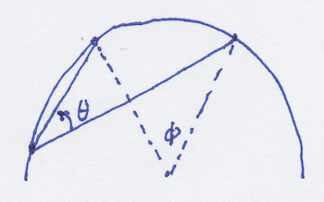
\includegraphics [scale=0.6] {D6.png} \end{center}

\emph{Proof}.

Label a few more angles.  Central angle $s$ and peripheral $t$ ($\angle BAC$) subtend the same arc of the circle.
\begin{center} 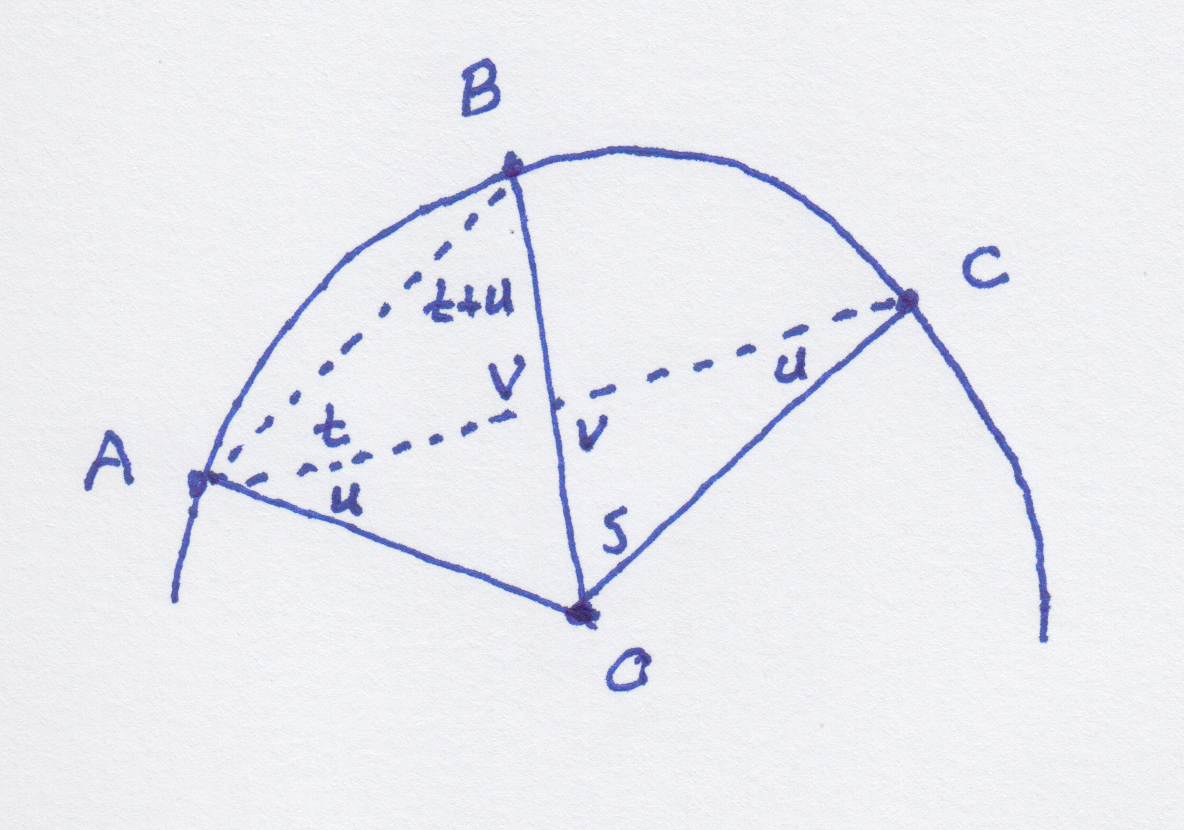
\includegraphics [scale=0.7] {D7.png} \end{center}

In isosceles $\triangle AOB$, the base angles of measure $t + u$ are equal.

In isosceles $\triangle AOC$, the base angles labeled $u$ are equal.  Furthermore, the angles labeled $v$ are vertical angles.

The triangle sum theorem says that
\[ t + t + u + v = s + u + v \]
\[ 2t = s \]

$\square$.

This proof is simple but not complete because the drawing assumes that the center of the triangle $O$ is not contained within the angle formed by $BAC$.  A more general proof by a similar construction is possible, but instead we introduce a different proof.
\begin{center} 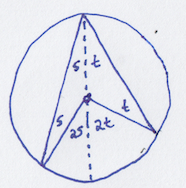
\includegraphics [scale=0.7] {D8.png} \end{center}

$s = s$ and $t = t$ by the isosceles triangle theorem.  Then the exterior angle theorem gives the central angles, and the sum gives our basic inscribed angle theorem.


\end{document}
